\begin{minipage}[b]{0.48\linewidth}
    \centering
    \small
    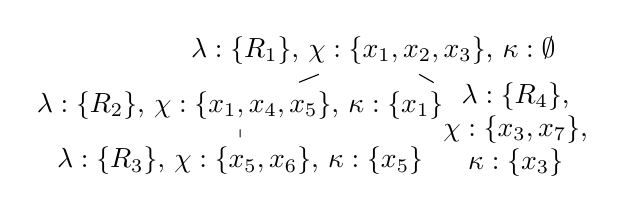
\begin{tikzpicture}[
			level distance=0.7cm,
			level 1/.style={sibling distance=3.5cm}
        ]
        \node[align=center] { $\lambda: \{ R_1 \}$, $\chi: \{ x_1, x_2, x_3 \}$, $\kappa: \emptyset$ }
            child[align=center] { node {$\lambda: \{ R_2 \}$, $\chi: \{ x_1, x_4, x_5 \}$, $\kappa: \{ x_1 \}$} edge from parent[-]
                child[align=center] { node {$\lambda: \{ R_3 \}$, $\chi: \{ x_5, x_6 \}$, $\kappa: \{ x_5 \}$} edge from parent[-] }
            }
            child[align=center,level distance=1cm] { node {$\lambda: \{ R_4 \} $,\\$\chi: \{ x_3, x_7 \}$,\\$\kappa: \{ x_3 \}$} edge from parent[-]
            } ;
    \end{tikzpicture}
    \captionof{figure}{Meta-decomposition of the query $Q_{\ref{ex:hierarchical}}$}
    \label{fig:hierarchical-meta}
\end{minipage}